\section{Tokenizing and Vocabulary}
Next, we tokenize the text data for that we created a custom RegexpTokenizer which tokenizes the text by only allowing words, numbers and some special characters. Even though the dataset is rather cleaned. Keeping exclasion marks and question marks can be useful for sentiment analysis. To see which words are most common in the dataset, we plot a WordCloud, which can be seen in Figure \ref{fig:wordcloud}.
\begin{figure}[H]
    \vspace*{0.7cm}
    \centering
    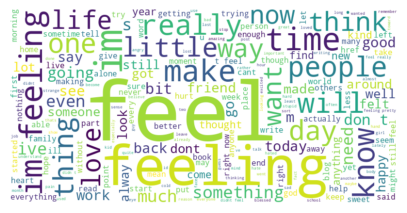
\includegraphics[width=0.4\textwidth]{figures/wordcloud.png}
    \caption{WordCloud of the vocabulary.}
    \label{fig:wordcloud}
    \vspace*{0.7cm}
\end{figure}
We see a clear tendency to words accoiated with...

To be sure also all the text was converted to lowercase. We then create a vocabulary of all the unique tokens in the dataset. The vocabulary is then used to convert the text data into sequences of integers. The vocabulary for the training dataset ended up being 15,212 words.

Hereafter, we need to determine the length of the sequences. We do this by plotting the distribution of the lengths of the sequences. The distribution given as a boxplot can be seen in Figure \ref{fig:sequence_length}.
\begin{figure}[H]
    \vspace*{0.7cm}
    \centering
    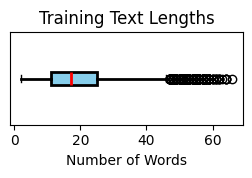
\includegraphics[width=0.22\textwidth]{figures/sentence_length.png}
    \caption{Distribution of the lengths of the sequences.}
    \label{fig:sequence_length}
    \vspace*{0.7cm}
\end{figure}
From the boxplot, we see that the majority of the sequences have a length of around 20 words. We choose to set the maximum sequence length to 23 words. This means that all sequences longer than 23 words are truncated, and all sequences shorter than 23 words are padded with a special token, '<PAD>', to make them all the same length.

